\section{Widgets (1)}\label{widgets-1}

\subsection{GtkLabel, GtkButton and
GtkBox}\label{gtklabel-gtkbutton-and-gtkbox}

\subsubsection{GtkLabel}\label{gtklabel}

We made a window and showed it on the screen in the previous section.
Now we go on to the next topic: widgets. The simplest widget is
GtkLabel. It is a widget with text in it.

\begin{lstlisting}[language=C, numbers=left]
#include <gtk/gtk.h>

static void
app_activate (GApplication *app) {
  GtkWidget *win;
  GtkWidget *lab;

  win = gtk_application_window_new (GTK_APPLICATION (app));
  gtk_window_set_title (GTK_WINDOW (win), "lb1");
  gtk_window_set_default_size (GTK_WINDOW (win), 400, 300);

  lab = gtk_label_new ("Hello.");
  gtk_window_set_child (GTK_WINDOW (win), lab);

  gtk_window_present (GTK_WINDOW (win));
}

int
main (int argc, char **argv) {
  GtkApplication *app;
  int stat;

  app = gtk_application_new ("com.github.ToshioCP.lb1", G_APPLICATION_DEFAULT_FLAGS);
  g_signal_connect (app, "activate", G_CALLBACK (app_activate), NULL);
  stat =g_application_run (G_APPLICATION (app), argc, argv);
  g_object_unref (app);
  return stat;
}
\end{lstlisting}

Save this program to a file \passthrough{\lstinline!lb1.c!}. (You can
use \passthrough{\lstinline!src/misc/lb1.c!} if you've downloaded this
repository.) Then compile and run it.

\begin{lstlisting}
$ comp lb1
$ ./a.out
\end{lstlisting}

A window with a message ``Hello.'' appears.

\begin{figure}
\centering
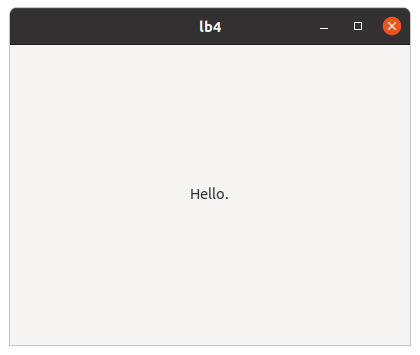
\includegraphics[width=6.3cm,height=5.325cm]{../image/screenshot_lb1.png}
\caption{Screenshot of the label}
\end{figure}

There are only a few changes between \passthrough{\lstinline!pr4.c!} and
\passthrough{\lstinline!lb1.c!}. A program
\passthrough{\lstinline!diff!} is useful to know the difference.

\begin{lstlisting}
$ cd misc; diff pr4.c lb1.c
4c4
< app_activate (GApplication *app, gpointer user_data) {
---
> app_activate (GApplication *app) {
5a6
>   GtkWidget *lab;
8c9
<   gtk_window_set_title (GTK_WINDOW (win), "pr4");
---
>   gtk_window_set_title (GTK_WINDOW (win), "lb1");
9a11,14
> 
>   lab = gtk_label_new ("Hello.");
>   gtk_window_set_child (GTK_WINDOW (win), lab);
> 
18c23
<   app = gtk_application_new ("com.github.ToshioCP.pr4", G_APPLICATION_DEFAULT_FLAGS);
---
>   app = gtk_application_new ("com.github.ToshioCP.lb1", G_APPLICATION_DEFAULT_FLAGS);
\end{lstlisting}

This tells us:

\begin{itemize}
\tightlist
\item
  A signal handler \passthrough{\lstinline!app\_activate!} doesn't have
  \passthrough{\lstinline!user\_data!} parameter. If the fourth argument
  of \passthrough{\lstinline!g\_signal\_connect!} is NULL, you can leave
  out \passthrough{\lstinline!user\_data!}.
\item
  The definition of a new variable \passthrough{\lstinline!lab!} is
  added.
\item
  The title of the window is changed.
\item
  A label is created and connected to the window as a child.
\end{itemize}

The function
\passthrough{\lstinline!gtk\_window\_set\_child (GTK\_WINDOW (win), lab)!}
makes the label \passthrough{\lstinline!lab!} a child widget of the
window \passthrough{\lstinline!win!}. Be careful. A child widget is
different from a child object. Objects have parent-child relationships
and widgets also have parent-child relationships. But these two
relationships are totally different. Don't be confused. In the program
\passthrough{\lstinline!lb1.c!}, \passthrough{\lstinline!lab!} is a
child widget of \passthrough{\lstinline!win!}. Child widgets are always
located in their parent widget on the screen. See how the window has
appeared on the screen. The application window includes the label.

The window \passthrough{\lstinline!win!} doesn't have any parents. We
call such a window top-level window. An application can have more than
one top-level windows.

\subsubsection{GtkButton}\label{gtkbutton}

The next widget is GtkButton. It displays a button on the screen with a
label or icon on it. In this subsection, we will make a button with a
label. When the button is clicked, it emits a ``clicked'' signal. The
following program shows how to catch the signal and do something.

\begin{lstlisting}[language=C, numbers=left]
#include <gtk/gtk.h>

static void
click_cb (GtkButton *btn) {
  g_print ("Clicked.\n");
}

static void
app_activate (GApplication *app) {
  GtkWidget *win;
  GtkWidget *btn;

  win = gtk_application_window_new (GTK_APPLICATION (app));
  gtk_window_set_title (GTK_WINDOW (win), "lb2");
  gtk_window_set_default_size (GTK_WINDOW (win), 400, 300);

  btn = gtk_button_new_with_label ("Click me");
  gtk_window_set_child (GTK_WINDOW (win), btn);
  g_signal_connect (btn, "clicked", G_CALLBACK (click_cb), NULL);

  gtk_window_present (GTK_WINDOW (win));
}

int
main (int argc, char **argv) {
  GtkApplication *app;
  int stat;

  app = gtk_application_new ("com.github.ToshioCP.lb2", G_APPLICATION_DEFAULT_FLAGS);
  g_signal_connect (app, "activate", G_CALLBACK (app_activate), NULL);
  stat =g_application_run (G_APPLICATION (app), argc, argv);
  g_object_unref (app);
  return stat;
}
\end{lstlisting}

Look at the line 17 to 19. First, it creates a GtkButton instance
\passthrough{\lstinline!btn!} with a label ``Click me''. Then, adds the
button to the window \passthrough{\lstinline!win!} as a child. Finally,
connects the ``clicked'' signal of the button to the handler
\passthrough{\lstinline!click\_cb!}. So, if
\passthrough{\lstinline!btn!} is clicked, the function
\passthrough{\lstinline!click\_cb!} is invoked. The suffix ``cb'' means
``call back''.

Name the program \passthrough{\lstinline!lb2.c!} and save it. Now
compile and run it.

\begin{figure}
\centering
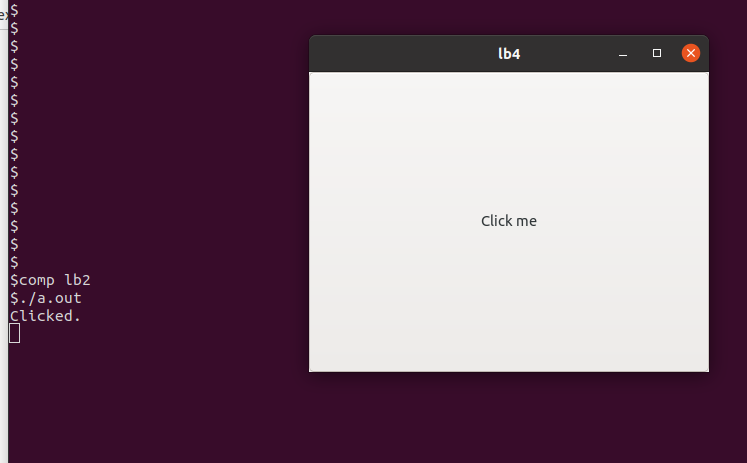
\includegraphics[width=11.205cm,height=6.945cm]{../image/screenshot_lb2.png}
\caption{Screenshot of the label}
\end{figure}

A window with the button appears. Click the button (it is a large
button, you can click everywhere in the window), then a string
``Clicked.'' appears on the terminal. It shows the handler was invoked
by clicking the button.

It's good that we've made sure that the clicked signal was caught and
the handler was invoked by using \passthrough{\lstinline!g\_print!}.
However, using \passthrough{\lstinline!g\_print!} is out of harmony with
GTK, which is a GUI library. So, we will change the handler. The
following code is extracted from \passthrough{\lstinline!lb3.c!}.

\begin{lstlisting}[language=C, numbers=left]
static void
click_cb (GtkButton *btn, GtkWindow *win) {
  gtk_window_destroy (win);
}

static void
app_activate (GApplication *app) {
  GtkWidget *win;
  GtkWidget *btn;

  win = gtk_application_window_new (GTK_APPLICATION (app));
  gtk_window_set_title (GTK_WINDOW (win), "lb3");
  gtk_window_set_default_size (GTK_WINDOW (win), 400, 300);

  btn = gtk_button_new_with_label ("Close");
  gtk_window_set_child (GTK_WINDOW (win), btn);
  g_signal_connect (btn, "clicked", G_CALLBACK (click_cb), win);

  gtk_window_present (GTK_WINDOW (win));
}
\end{lstlisting}

And the difference between \passthrough{\lstinline!lb2.c!} and
\passthrough{\lstinline!lb3.c!} is as follows.

\begin{lstlisting}
$ cd misc; diff lb2.c lb3.c
4,5c4,5
< click_cb (GtkButton *btn) {
<   g_print ("Clicked.\n");
---
> click_cb (GtkButton *btn, GtkWindow *win) {
>   gtk_window_destroy (win);
14c14
<   gtk_window_set_title (GTK_WINDOW (win), "lb2");
---
>   gtk_window_set_title (GTK_WINDOW (win), "lb3");
17c17
<   btn = gtk_button_new_with_label ("Click me");
---
>   btn = gtk_button_new_with_label ("Close");
19c19
<   g_signal_connect (btn, "clicked", G_CALLBACK (click_cb), NULL);
---
>   g_signal_connect (btn, "clicked", G_CALLBACK (click_cb), win);
29c29
<   app = gtk_application_new ("com.github.ToshioCP.lb2", G_APPLICATION_DEFAULT_FLAGS);
---
>   app = gtk_application_new ("com.github.ToshioCP.lb3", G_APPLICATION_DEFAULT_FLAGS);
35d34
< 
\end{lstlisting}

The changes are:

\begin{itemize}
\tightlist
\item
  The function \passthrough{\lstinline!g\_print!} in
  \passthrough{\lstinline!lb2.c!} was deleted and two lines are
  inserted.

  \begin{itemize}
  \tightlist
  \item
    \passthrough{\lstinline!click\_cb!} has the second parameter, which
    comes from the fourth argument of the
    \passthrough{\lstinline!g\_signal\_connect!} at line 17. One thing
    to be careful is the types are different between the second
    parameter of \passthrough{\lstinline!click\_cb!} and the fourth
    argument of \passthrough{\lstinline!g\_signal\_connect!}. The former
    is \passthrough{\lstinline!GtkWindow *!} and the latter is
    \passthrough{\lstinline!GtkWidget *!}. The compiler doesn't complain
    because \passthrough{\lstinline!g\_signal\_connect!} uses gpointer
    (general type of pointer). In this program the instance pointed by
    \passthrough{\lstinline!win!} is a GtkApplicationWindow object. It
    is a descendant of GtkWindow and GtkWidget class, so both
    \passthrough{\lstinline!GtkWindow *!} and
    \passthrough{\lstinline!GtkWidget *!} are correct types of the
    instance.
  \item
    \passthrough{\lstinline!gtk\_destroy (win)!} destroys the top-level
    window. Then the application quits.
  \end{itemize}
\item
  The label of \passthrough{\lstinline!btn!} is changed from ``Click
  me'' to ``Close''.
\item
  The fourth argument of \passthrough{\lstinline!g\_signal\_connect!} is
  changed from \passthrough{\lstinline!NULL!} to
  \passthrough{\lstinline!win!}.
\end{itemize}

The most important change is the fourth argument of the
\passthrough{\lstinline!g\_signal\_connect!}. This argument is described
as ``data to pass to the handler'' in the definition of
\href{https://docs.gtk.org/gobject/func.signal_connect.html}{\passthrough{\lstinline!g\_signal\_connect!}}.

\subsubsection{GtkBox}\label{gtkbox}

GtkWindow and GtkApplicationWindow can have only one child. If you want
to add two or more widgets in a window, you need a container widget.
GtkBox is one of the containers. It arranges two or more child widgets
into a single row or column. The following procedure shows the way to
add two buttons in a window.

\begin{itemize}
\tightlist
\item
  Create a GtkApplicationWindow instance.
\item
  Create a GtkBox instance and add it to the GtkApplicationWindow as a
  child.
\item
  Create a GtkButton instance and append it to the GtkBox.
\item
  Create another GtkButton instance and append it to the GtkBox.
\end{itemize}

After this, the Widgets are connected as the following diagram.

\begin{figure}
\centering
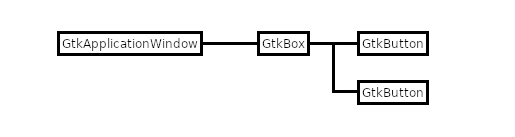
\includegraphics[width=7.725cm,height=2.055cm]{../image/box.png}
\caption{Parent-child relationship}
\end{figure}

The program \passthrough{\lstinline!lb4.c!} is as follows.

\begin{lstlisting}[language=C, numbers=left]
#include <gtk/gtk.h>

static void
click1_cb (GtkButton *btn) {
  const char *s;

  s = gtk_button_get_label (btn);
  if (g_strcmp0 (s, "Hello.") == 0)
    gtk_button_set_label (btn, "Good-bye.");
  else
    gtk_button_set_label (btn, "Hello.");
}

static void
click2_cb (GtkButton *btn, GtkWindow *win) {
  gtk_window_destroy (win);
}

static void
app_activate (GApplication *app) {
  GtkWidget *win;
  GtkWidget *box;
  GtkWidget *btn1;
  GtkWidget *btn2;

  win = gtk_application_window_new (GTK_APPLICATION (app));
  gtk_window_set_title (GTK_WINDOW (win), "lb4");
  gtk_window_set_default_size (GTK_WINDOW (win), 400, 300);

  box = gtk_box_new (GTK_ORIENTATION_VERTICAL, 5);
  gtk_box_set_homogeneous (GTK_BOX (box), TRUE);
  gtk_window_set_child (GTK_WINDOW (win), box);

  btn1 = gtk_button_new_with_label ("Hello.");
  g_signal_connect (btn1, "clicked", G_CALLBACK (click1_cb), NULL);

  btn2 = gtk_button_new_with_label ("Close");
  g_signal_connect (btn2, "clicked", G_CALLBACK (click2_cb), win);

  gtk_box_append (GTK_BOX (box), btn1);
  gtk_box_append (GTK_BOX (box), btn2);

  gtk_window_present (GTK_WINDOW (win));
}

int
main (int argc, char **argv) {
  GtkApplication *app;
  int stat;

  app = gtk_application_new ("com.github.ToshioCP.lb4", G_APPLICATION_DEFAULT_FLAGS);
  g_signal_connect (app, "activate", G_CALLBACK (app_activate), NULL);
  stat =g_application_run (G_APPLICATION (app), argc, argv);
  g_object_unref (app);
  return stat;
}
\end{lstlisting}

Look at the function \passthrough{\lstinline!app\_activate!}.

After the creation of a GtkApplicationWindow instance, a GtkBox instance
is created.

\begin{lstlisting}[language=C]
box = gtk_box_new(GTK_ORIENTATION_VERTICAL, 5);
gtk_box_set_homogeneous (GTK_BOX (box), TRUE);
\end{lstlisting}

The first argument arranges the children of the box vertically. The
orientation constants are defined like this:

\begin{itemize}
\tightlist
\item
  GTK\_ORIENTATION\_VERTICAL: the children widgets are arranged
  vertically
\item
  GTK\_ORIENTATION\_HORIZONTAL: the children widgets are arranged
  horizontally
\end{itemize}

The second argument is the size of the space between the children. The
unit of the length is pixel.

The next function fills the box with the children, giving them the same
space.

After that, two buttons \passthrough{\lstinline!btn1!} and
\passthrough{\lstinline!btn2!} are created and the signal handlers are
set. Then, these two buttons are appended to the box.

\begin{lstlisting}[language=C, numbers=left]
static void
click1_cb (GtkButton *btn) {
  const char *s;

  s = gtk_button_get_label (btn);
  if (g_strcmp0 (s, "Hello.") == 0)
    gtk_button_set_label (btn, "Good-bye.");
  else
    gtk_button_set_label (btn, "Hello.");
}
\end{lstlisting}

The function \passthrough{\lstinline!gtk\_button\_get\_label!} returns a
text from the label. The string is owned by the button and you can't
modify or free it. The \passthrough{\lstinline!const!} qualifier is
necessary for the string \passthrough{\lstinline!s!}. If you change the
string, your compiler will give you a waring.

You always need to be careful with the const qualifier when you see the
GTK 4 API reference.

\begin{figure}
\centering
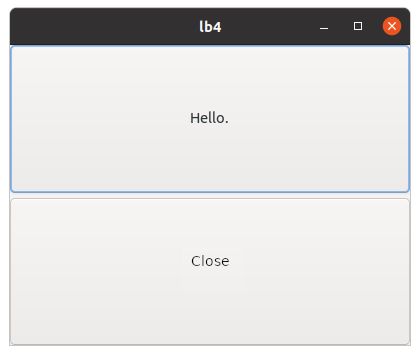
\includegraphics[width=6.3cm,height=5.325cm]{../image/screenshot_lb4.png}
\caption{Screenshot of the box}
\end{figure}

The handler corresponding to \passthrough{\lstinline!btn1!} toggles its
label. The handler corresponding to \passthrough{\lstinline!btn2!}
destroys the top-level window and the application quits.
